Determining the water density in the beam at the ion trap is more difficult than in the CBGB and stem region. During normal operation of the CBGB, the RGA in the trap chamber, which is off the beam axis and in a nipple, is unable to detect a change in the background water pressure. We turn to the trapped ions to find an answer.

By introducing water via the CBGB into the chamber with laser cooled \ce{Be+} ions, we observe reactions \ref{r: Be(S)+H2O->BeOH} and \ref{r: Be(P)+H2O->BeOH} from delayed TOF traces. Knowing the rate constant for this reaction (equation \ref{eq: k Be+H2O(T)}), we may find the density of the beam. The reaction products are ejected from the trap into the time of flight mass spectrometer (TOF-MS) at various delay times and the integrated ion signal is recorded. Assuming a forward velocity for \ce{H2O} upwards of 200 m/s, we have a reaction temperature of $\approx$20 K. The interaction produces reactions \ref{r: Be(S)+H2O->BeOH} and \ref{r: Be(P)+H2O->BeOH}, which were experimentally determined to react at temperature ($T$) and \ce{^2P3/2} state excitation fraction ($P$) at a rate defined by equation \ref{eq: k Be+H2O(T)}.

\begin{figure}[H]
	\centering
	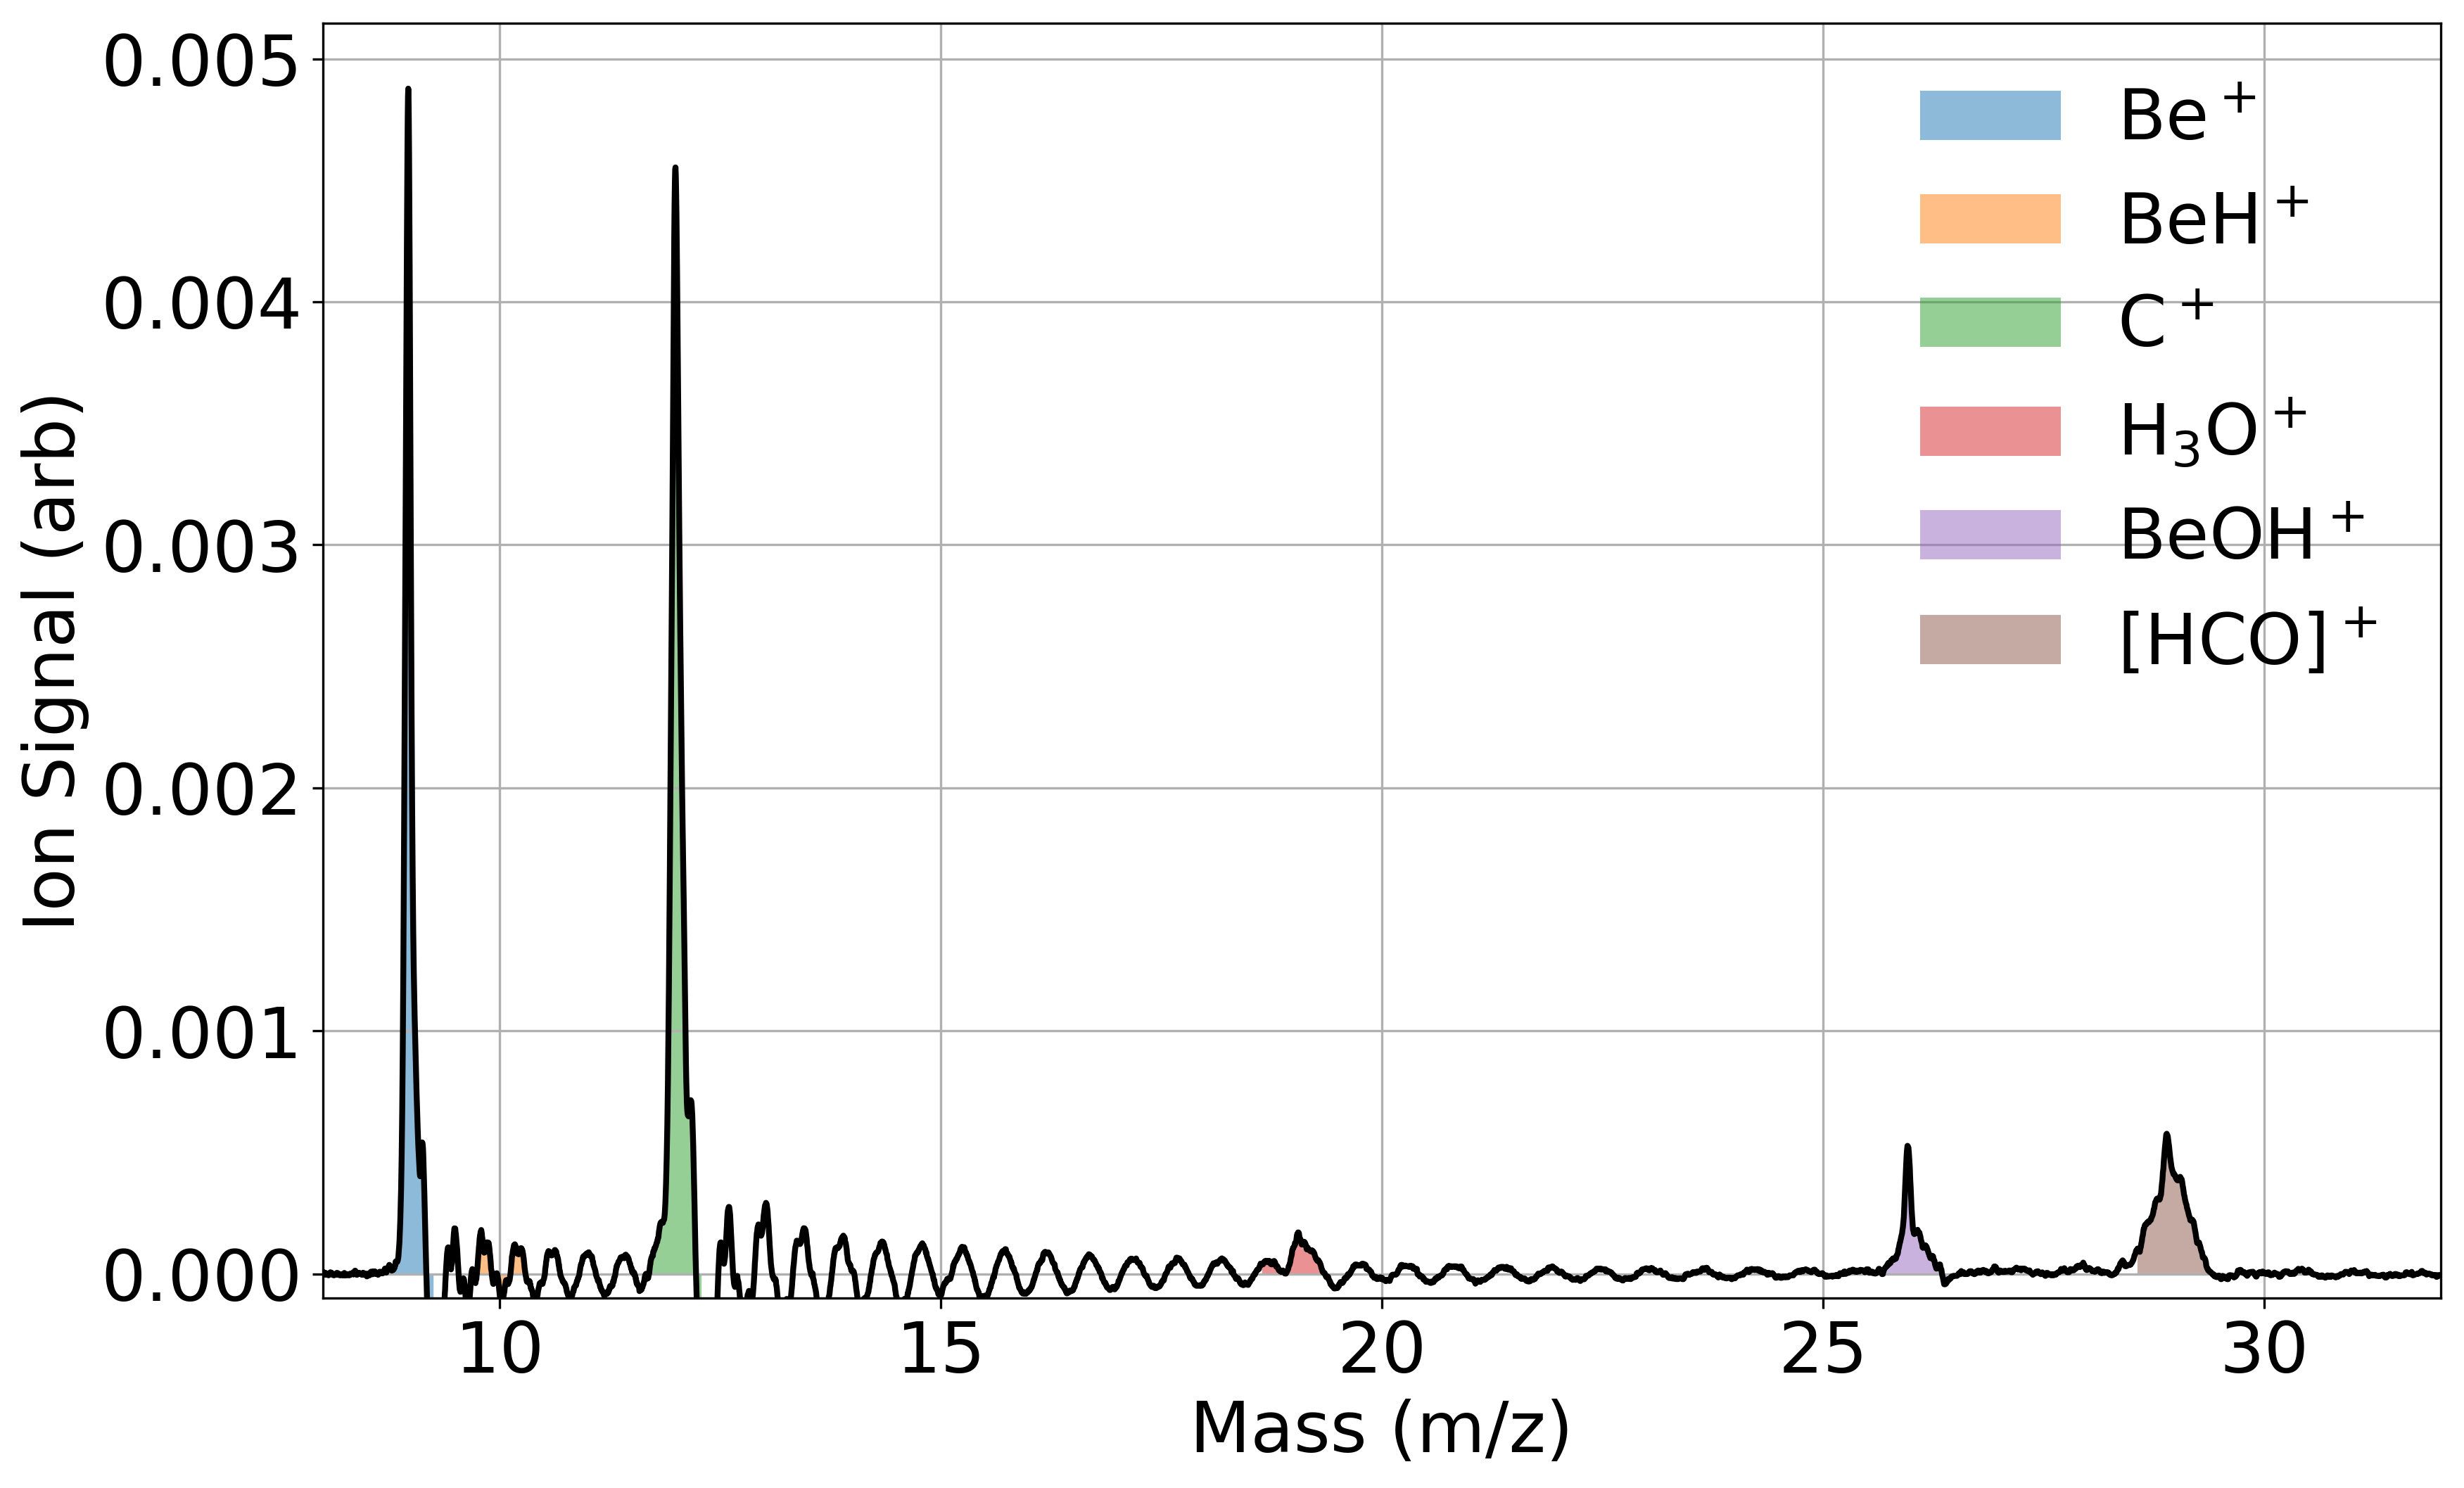
\includegraphics[width=0.8\textwidth]{images/C_H2O_beam_TOF.png}
	\caption{text}
	\label{fig: Be C H2O beam TOF}
\end{figure}

\begin{figure}[H]
	\centering
	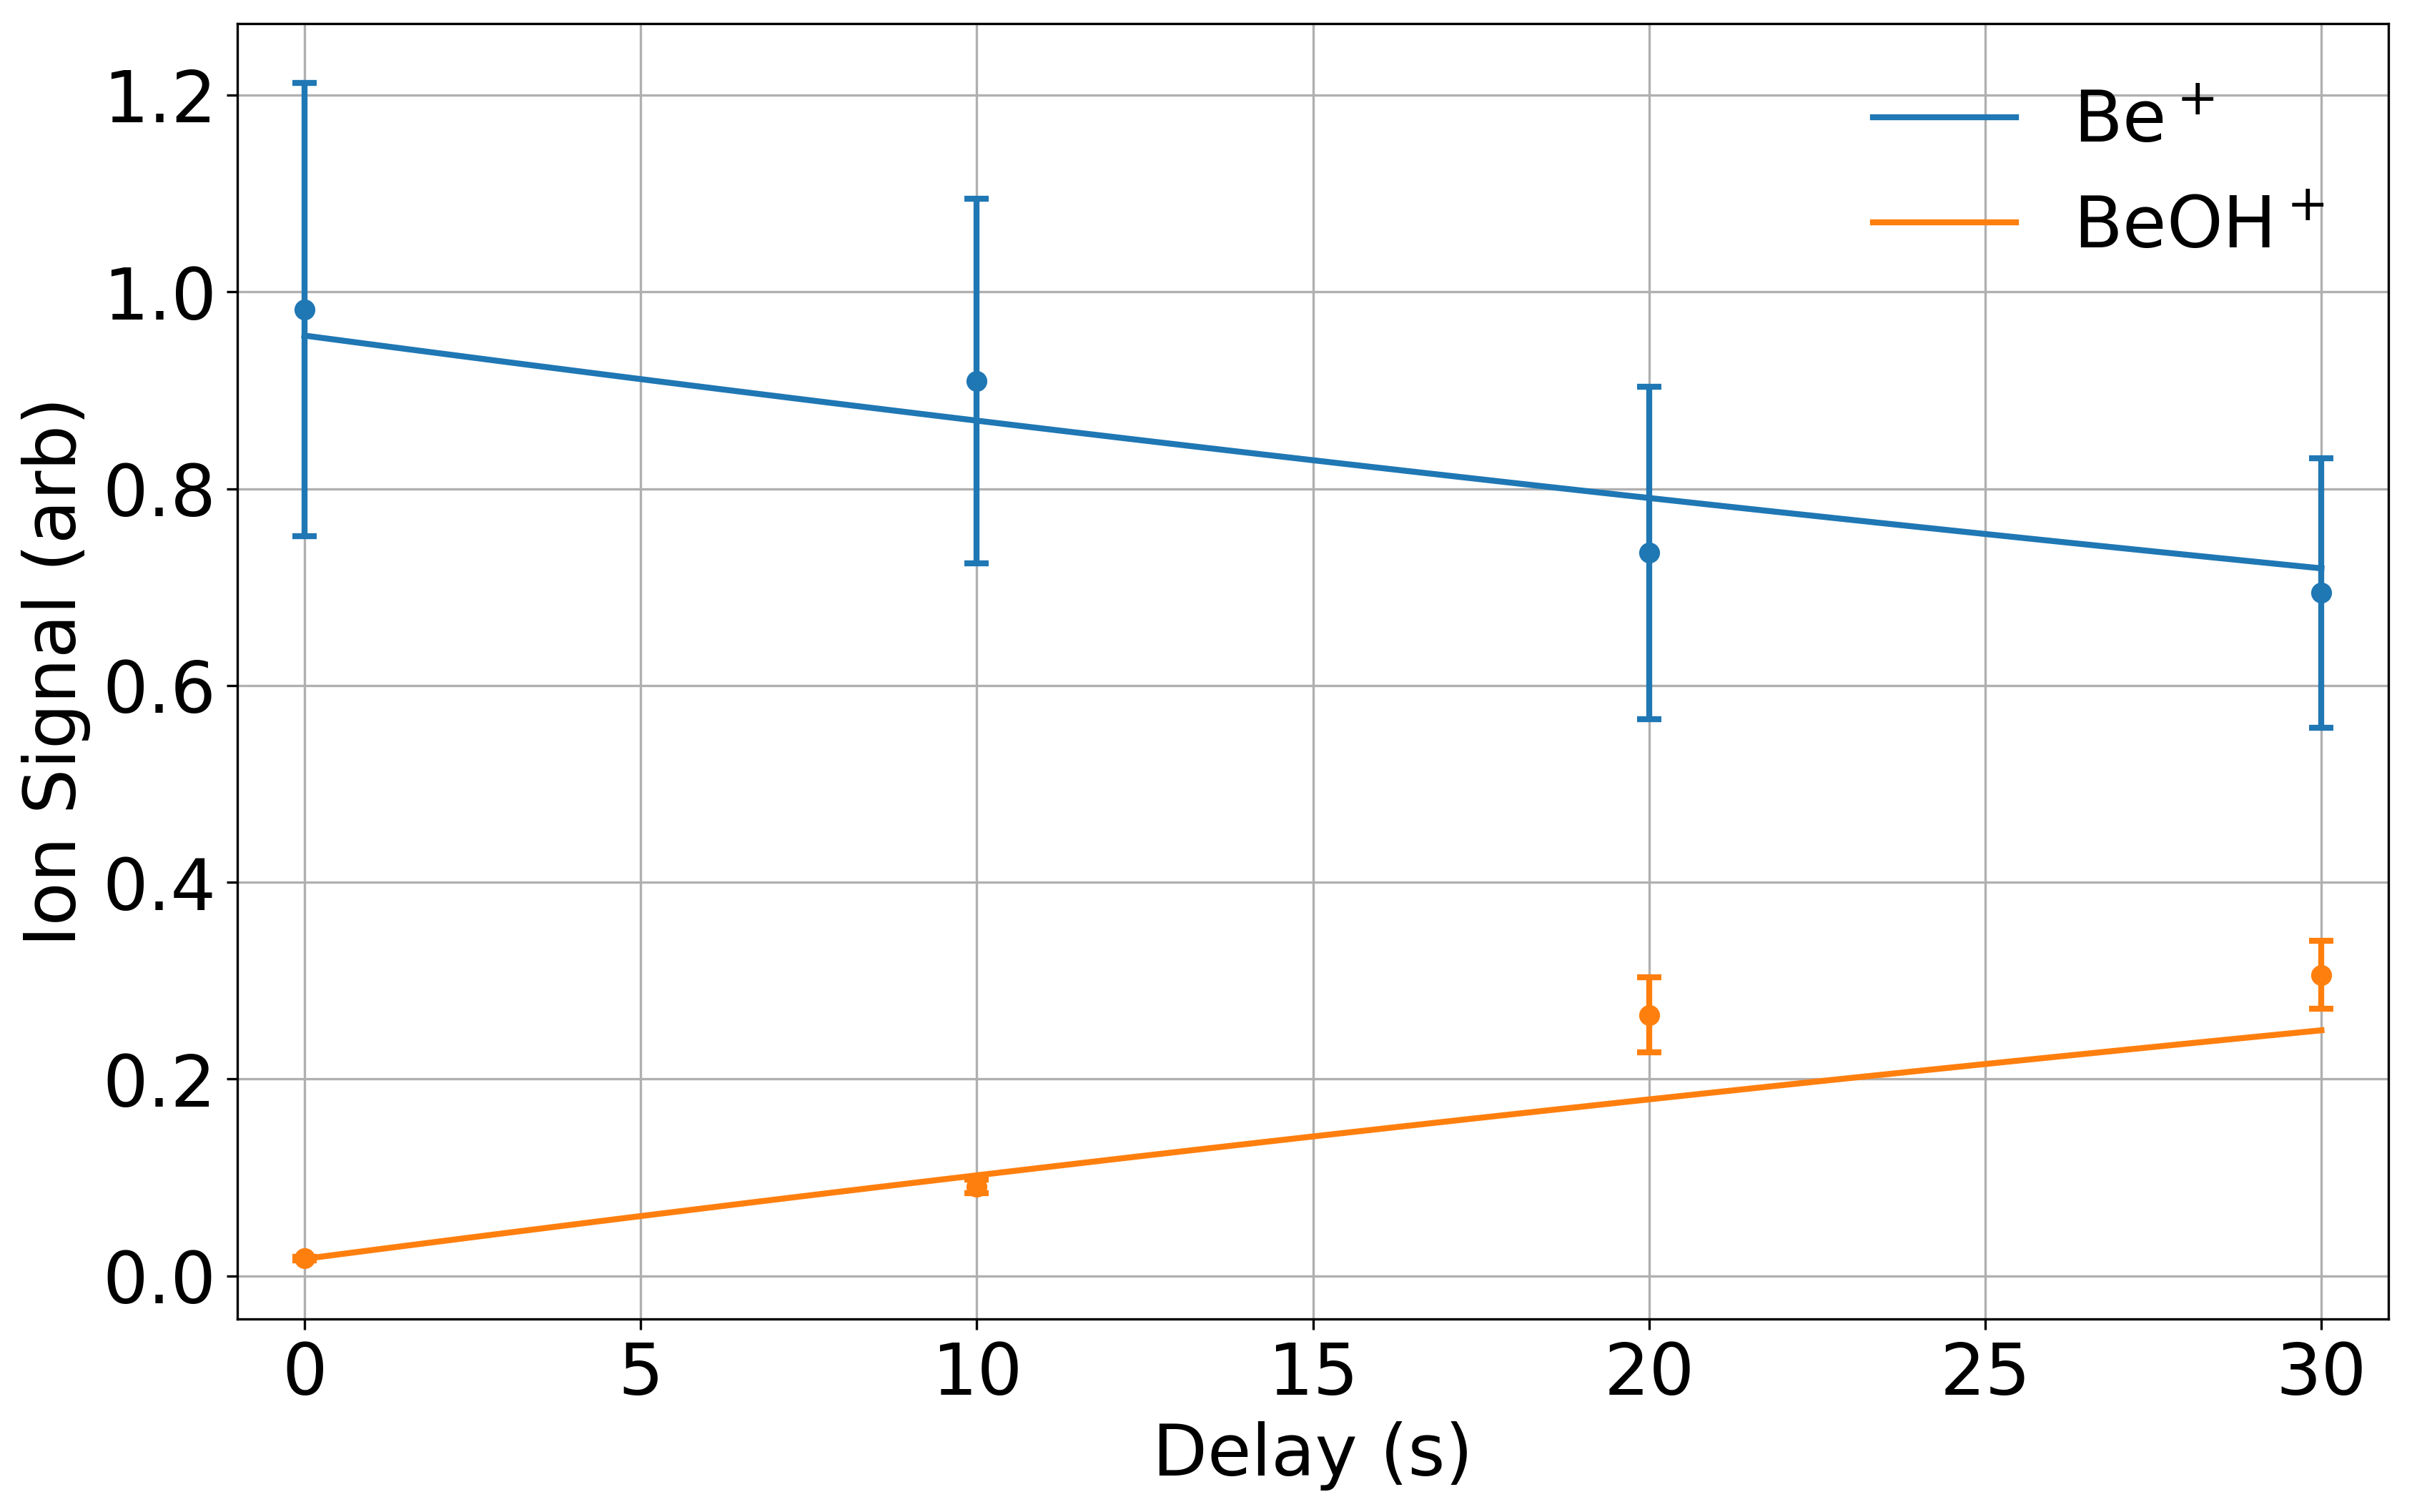
\includegraphics[width=0.8\textwidth]{images/Be_H2O_beam_traces.png}
	\caption{\ce{Be+} decay and \ce{BeOH+} appearance due to the introduction of \ce{H2O} from the CBGB. A shared fit of rates \ref{r: Be(S)+H2O->BeOH} and \ref{r: Be(P)+H2O->BeOH} yields a water beam density $\rho_{beam} = (2.18 \pm 0.37) \times 10^6$ cm$^{-3}$.}
%	Reduced chi square of 2
	\label{fig: Be H2O beam}
\end{figure}

Using the ADO approximation

\todo{Write this after Be+H2O is done}